\chapter{Architettura del Sistema}
\label{cap:architettura}
\thispagestyle{empty}

\begin{quotation}
{\footnotesize
\noindent \emph{}
\begin{flushright}
\end{flushright}
}
\end{quotation}
\vspace{0.5cm}

\section{Introduzione}

In questo capitolo descriveremo l'architettura del sistema implementato. Il sistema è stato progettato in maniera modulare per una serie di motivi: questo tipo di architettura permette di riutilizzare i moduli sviluppati, di estendere semplicemente il sistema con altri moduli, di sostituire eventualmente un intero modulo con un altro che compia le stesse funzioni, di comunicare in maniera semplice con altri sistemi. 

Per raggiungere questo scopo, si è deciso quindi di utilizzare il middleware ROS (Robot Operating System)~\cite{quigley2009ros}.
ROS è un middleware che, oltre ad offrire molti strumenti utili per lo sviluppo di complesse applicazioni robotiche, implementa due pattern architetturali importanti, entrambi usati nel nostro lavoro: il pattern publish-subscribe e il pattern client-server.
Questi due pattern sono implementati rispettivamente tramite messaggi e servizi: i messaggi definiscono un formato comune per la pubblicazione di dati in topic, i servizi invece specificano un'interfaccia per le chiamate a procedure remote, dichiarando gli input e gli output tra client e server.
Ogni processo che viene eseguito in ROS è chiamato nodo. Per eseguire qualsiasi sistema basato su ROS, devono essere presenti tre ulteriori nodi: il nodo Master, che si occupa di garantire la comunicazione tra gli altri nodi, tramite i due pattern supportati, il server dei parametri, che implementa un dizionario condiviso accessibile tramite la rete, in cui i nodi possono memorizzare e recuperare parametri usati dai loro algoritmi a runtime, il nodo rosout, che si occupa di mantenere i log prodotti dalle applicazioni.

Il sistema sviluppato è pensato per interagire con qualsiasi tipo di robot che sia provvisto di una videocamera monoculare e una unità di misura inerziale (IMU) tramite le due interfacce standard di ROS.
Esse consistono in tre topic: ``imu'', per i dati provenienti dall'unità di misura inerziale, ``image\_raw'', per l'immagine proveniente dalla videocamera, ``camera\_info'', che contiene i parametri intrinseci della videocamera, tra cui la matrice di calibrazione della videocamera utilizzata, necessaria per il funzionamento del sistema.
I dati estratti dall'unità di misura inerziale devono poter essere riferiti al sistema di coordinate della videocamera, infatti l'algoritmo di visione implementato utilizza i dati provenienti dalla IMU per stimare approssimativamente la posa della telecamera.
Per rendere l'algoritmo portabile, si utilizza a libreria tf di ROS. La libreria tf gestisce le trasformazioni da sistema di coordinate all'altro, pubblicando un albero di trasformazioni nel topic ``tf''.
Negli header dei messaggi standard di ROS è definito il campo ``frame\_id'', che descrive il nome del sistema di coordinate rispetto al quale è riferito il contenuto del messaggio. Grazie a questo, è possibile riferire i dati della IMU rispetto alle coordinate dell'immagine, purché sia nota la trasformazione tra i due frame.

\section{Diagramma del sistema}

L'architettura del sistema implementato è descritta in \autoref{fig:architettura-sistema}. \\
\begin{figure}[h]
  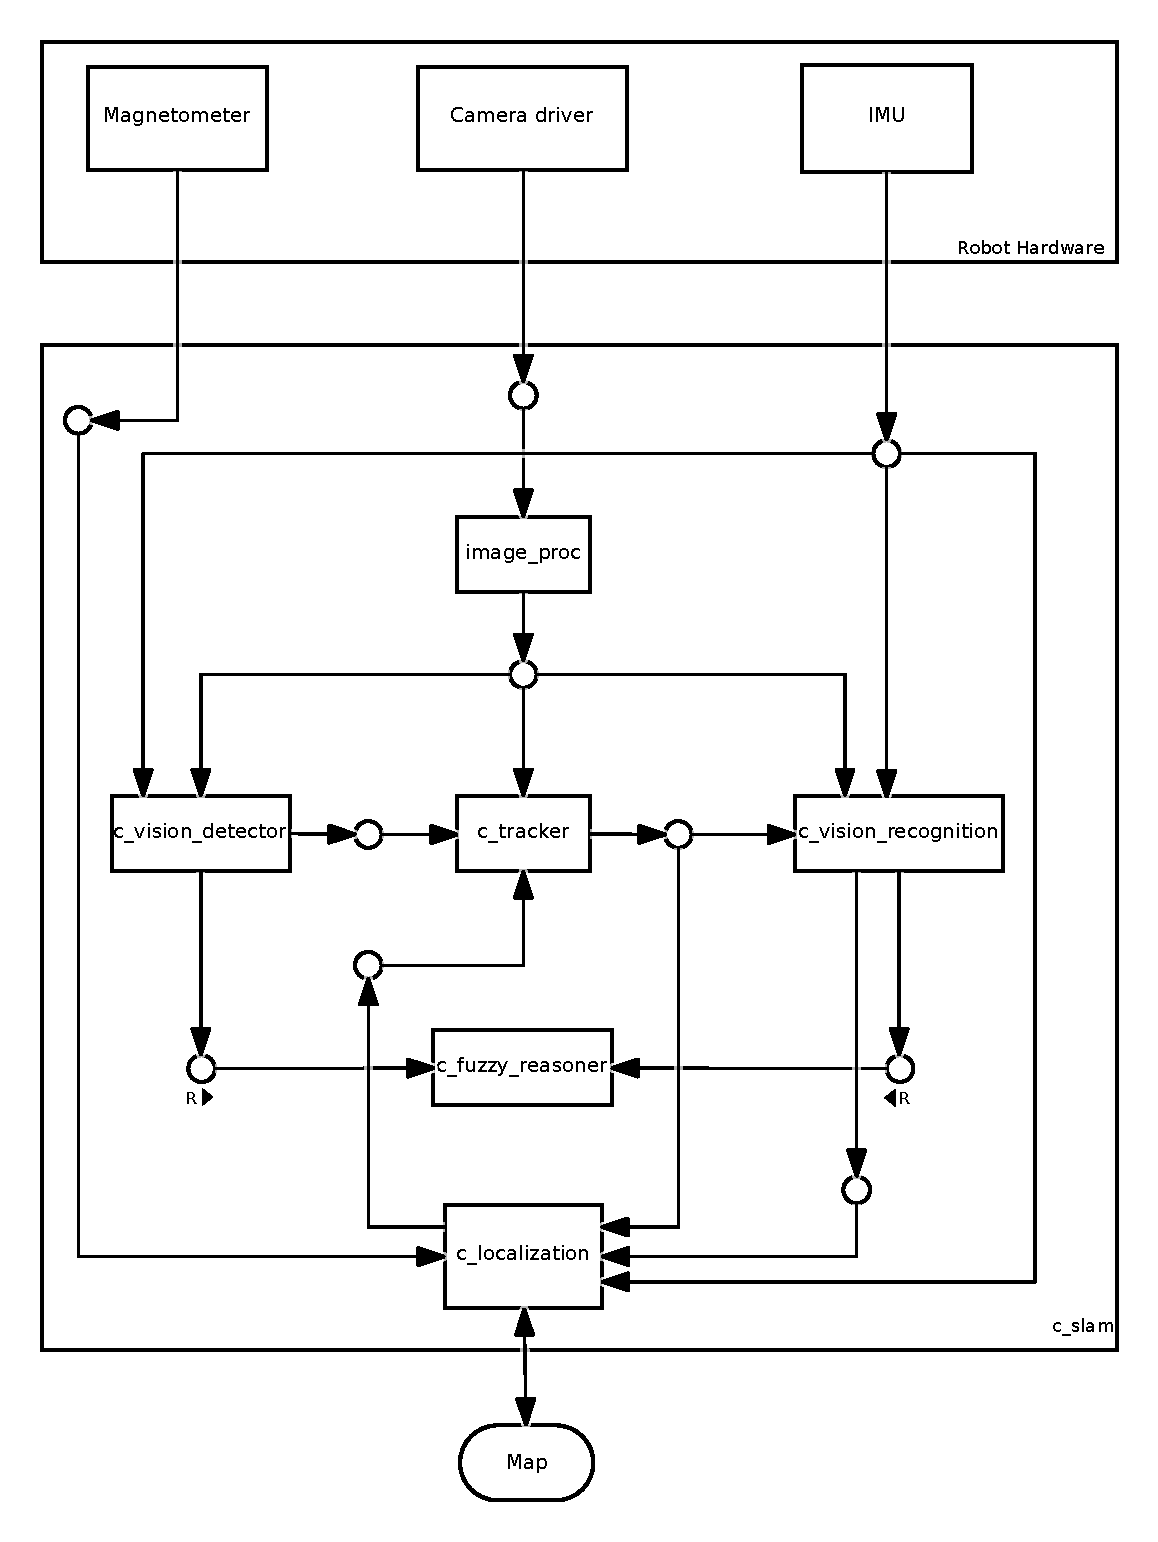
\includegraphics[width=0.9\textwidth]{diagrammi/Sistema}
  \caption{Architettura del sistema implementato}
  \label{fig:architettura-sistema}
\end{figure}


Il diagramma rappresenta i nodi del sistema, segue una breve descrizione di ogni elemento per specificare la loro funzione:

\begin{description}
  \item [image\_proc] si occupa di eliminare la distorsione radiale della videocamera causata dalla curvatura della lente.
  \item [c\_vision\_detector] si occupa di estrarre possibili feature dall'immagine.
  \item [c\_tracking] si occupa di seguire le feature a basso livello estratte dal nodo ``c\_vision\_detector'' nell'immagine, mantenendo un modello in modo da riuscire a riconoscere la feature anche dopo essere stata persa. 
  \item [c\_vision\_slam] si occupa dell'analisi approfondita delle feature, in modo da determinare il tipo di oggetto e la sua posizione nello spazio. 
  \item [c\_fuzzy\_reasoner] implementa un reasoner fuzzy; data una base di conoscenza e un classificatore, analizza le feature in ingresso e le classifica. 
\end{description}


\section{Comunicazione tra i nodi}

Questo sistema sfrutta sia il paradigma client-server, per l'interazione con il reasoner, che il paradigma publish-subscribe, in tutti gli altri casi.
Il reasoner offre 4 servizi:

\begin{description}
 \item [\/reasoning] questo servizio è un normale servizio di reasoning basato su una knowledgebase fuzzy.
 \item [\/classification] questo servizio si occupa di classificare istanze di feature riconosciute.
 \item [\/getDependencyGraph] questo servizio restituisce il grafo delle dipendenze del classificatore.
 \item [\/getReasoningGraph] questo servizio restituisce il grafo di reasoning utilizzato dal classificatore.
\end{description}

Il reasoner e i suoi servizi verranno discussi approfonditamente  nel \autoref{cap:reasoning}.

le informazioni riguardanti gli oggetti riconosciuti e seguiti dal sistema sono scambiate tramite i seguenti topic:

\begin{description}
 \item [\/to\_track] in questo topic vengono pubblicate le possibili feature riconosciute dall'intera immagine. Viene fornito il contorno della feature e la sua possibile classificazione.
 \item [\/tracks] in questo topic vengono pubblicati i risultati dell'algoritmo di tracking: contiene il bounding box e il contorno della feature, quest'ultimo viene maggiorato del 20\%, per assicurarsi di mantenere all'interno di esso il reale contorno della feature.
\end{description}

Il riconoscimento di feature viene descritto nel \autoref{cap:riconoscimento}, il tracking delle feature riconosciute nel \autoref{cap:tracking}, e infine l'analisi ad alto livello viene effettuata nel \autoref{cap:mapping}.

\section{Parametri degli algoritmi}

Gli algoritmi utilizzati nel sistema, in particolare gli algoritmi di visione, hanno alcuni parametri che è possibile tarare per adattare il sistema a qualsiasi tipo di robot utilizzato.
Per gestire i parametri abbiamo utilizzato il server dei parametri di ROS.
Il server dei parametri è un dizionario, ossia ogni parametro, identificato da una stringa, è salvato nel server dei parametri, e può essere recuperato tramite il suo nome. 
Il server dei parametri supporta dizionari gerarchici, in modo da poter rappresentare tipi di dati strutturati. 
Inoltre è possibile definire parametri privati per qualsiasi nodo. I parametri privati restano accessibili da tutto il resto del sistema, ma nel dizionario vengono salvati sotto il nome del nodo a cui appartengono; questo comportamento è studiato per evitare collisioni tra parametri con lo stesso nome in nodi differenti.

Visto che gli algoritmi di estrazione e analisi delle feature si basano fortemente sugli stessi strumenti, questo sistema usa in maniera estesa i parametri privati, in modo da avere lo stesso parametro, che rappresenta concettualmente la stessa quantità, differente in base al nodo che lo utilizza.

Il sistema permette anche di cambiare i parametri a runtime, essi vengono aggiornati nei nodi che ne fanno uso con una frequenza fissa.
Si possono conoscere i parametri usati dal sistema e il loro significato nell'\autoref{app:manuale}.




